%%%%%%%%%%%%%%%%%%%%%%%%%%%%%%%%%%%%%%%%%
% Shisham's Templeate
%%%%%%%%%%%%%%%%%%%%%%%%%%%%%%%%%%%%%%%%%

%\documentclass{beamer}
%\mode<presentation> {
%\usetheme{Singapore}
%\usecolortheme{rose}
%}
%\usepackage{graphicx}
%\usepackage{booktabs} 
%\usepackage{pgfpages}
%\setbeamertemplate{footline}[frame number]
%\newcommand\identity{1\kern-0.25em\text{l}}


%%%%%%%%%%%%%%%%%%%%%%%%%%%%%%%%%%%%%%%%%
% Thanasis' Templeate
%%%%%%%%%%%%%%%%%%%%%%%%%%%%%%%%%%%%%%%%%

\documentclass[9pt,xcolor={svgnames}]{beamer}

\mode<presentation> {

\usetheme{default}

%\setbeamertemplate{footline} % To remove the footer line in all slides uncomment this line
\setbeamertemplate{footline}[frame number] % To replace the footer line in all slides with a simple slide count uncomment this line
\setbeamertemplate{footline}
{
  \hfill%
  \usebeamercolor[fg]{page number in head/foot}%
  \usebeamerfont{page number in head/foot}%
%  \insertframenumber\,/\,\inserttotalframenumber\kern1em\vskip2pt % original code
  \tiny % font size: tiny(default)/scriptsize/footnotesize/small/normalsize/large
  \insertframenumber
  \kern1em  % adjust the space on the right-hand side of the frame number
  \vskip4pt % adjust the space below the frame number
}

\setbeamertemplate{navigation symbols}{} % To remove the navigation symbols from the bottom of all slides uncomment this line
}

\usepackage{graphicx} % Allows including images
\usepackage{booktabs} % Allows the use of \toprule, \midrule and \bottomrule in tables
\usepackage{multicol}
\usepackage{mathtools}
\usepackage{geometry}
\usepackage{bbm}

\usepackage[export]{adjustbox}



\setbeamertemplate{itemize items}[circle]
\setbeamertemplate{itemize subitem}[default]
%\setbeamertemplate{enumerate items}[circle]\\
%\setbeamertemplate{items}[circle]

%\setbeamercolor{item}{fg=black} % all frames will have bullets with this color
%\setbeamercolor{caption name}{fg=gray} % all frames will have captions with this color

\usefonttheme[onlymath]{serif}

\setlength{\leftmargini}{9pt}
\setbeamersize{text margin left=20pt,text margin right=20pt}
%\setbeamerfont{institute}{size=\normalsize}

\setbeamertemplate{frametitle}
{
{\vskip  .6em} 
{\hskip -.35em}
\underline{\insertframetitle\vphantom{j}}
{\vskip -.6em}
}

\graphicspath{{./figs181007/}}

%----------------------------------------------------------------------------------------
%	TITLE PAGE
%----------------------------------------------------------------------------------------

\title[Short title]{\large \textbf{How much work experience do you need to get your first job? \\ \normalsize The macroeconomic implications of bias against labor market entrants}}
%\author[Author1, Author2, Author3]{Shisham Adhikari\inst{1} \and Athanasios Geromichalos\inst{2} \\ \and Ioannis Kospentaris\inst{3}}
%\institute[University A, University B, University C]{\inst{1} University of California - Davis\\ \email{shadhikari@ucdavis.edu} \and \inst{2} University of California - Davis\\ \email{ageromich@ucdavis.edu} \and \inst{3} Virginia Commonwealth University\\ \email{ikospentaris@vcu.edu}}
\author{Shisham Adhikari\thanks{\;University of California - Davis; email: \texttt{shadhikari@ucdavis.edu}} \and Athanasios Geromichalos\thanks{\;University of California - Davis; email: \texttt{ageromich@ucdavis.edu}} \and Ate\c{s} G\"ursoy \thanks{\;University of California - Davis; email: \texttt{agursoy@ucdavis.edu}} \and \\ Ioannis Kospentaris\thanks{\;Athens University of Economics and Business; email: \texttt{ikospentaris@aueb.gr}}}

\date[2024]{November 15, 2024\\[2mm]University of Ottawa}
%\date{\today}
% Presentations: West Coast SaM, UC Davis, University of Cyprus, CRETE, Athens Econ Winter Workshop, Mannheim, Midwest Macro, University of Ottawa, Vilnius SaM

\begin{document}

\begin{frame}
\titlepage % Print the title page as the first slide
\end{frame}

%===============================================
\section{Introduction} 
%===============================================

\begin{frame}{Motivation I}
A vicious circle (meme found in social media)...
\begin{figure}
        \centering
        
\includegraphics[scale=0.2]{motivation.png}
        \end{figure}
\end{frame}

\begin{frame}{Motivation II}
\begin{itemize}
\setlength\itemsep{1.8em} 
    \item The first step in a worker's career often is particularly hard
    \begin{itemize}
    \smallskip
    \item Job-finding rate for entrants is roughly half of the other unemployed 
    \hyperlink{jfr}{\beamerbutton{JFRs}} 
     \hypertarget{flow_jfr}{}
    \item 35\% of entry level positions posted since 2017 on LinkedIn require minimum three years of experience
    \item 43\% of college graduates start their career with a job that does not require a college degree
    %\item There has been a 20\% increase in the number of skills required on job listings since 2017
    \end{itemize}

    \item \textit{All} workers in the economy begin their career as labor market entrants

    \item Large literature documents that early-career shocks have long-lasting effects (von Wachter, 2020)

    \item Questions:
    \smallskip
    \begin{enumerate}
    %\item Why do firms avoid hiring inexperienced workers?
    \item What are the aggregate implications of firms' preference for experienced workers?
    \item Is there room for welfare-improving government interventions?
    \end{enumerate}
\end{itemize}
\end{frame}

%\begin{frame}{Research Question}
%\begin{itemize}
 %   \item What are the \textbf{aggregate welfare implications} of this exclusion of inexperienced workers, given that, by definition, all workers in the economy start their careers as inexperienced?
  %  \item What are the possible welfare improving government intervention?
%\end{itemize}
%\note{ In this paper, the authors }
%\end{frame}

\begin{frame}{What we do}
\begin{itemize}
\setlength\itemsep{2em}
    \item Build a DMP model with entrants and experienced workers
    \smallskip
    \begin{itemize}
    \item Firms that hire new workers have to incur training expenses
    \item New workers who stay unemployed for an extended time period suffer skill loss
    \end{itemize}

  %  \item Firms who employ new workers provide a public good to society
   % \smallskip
    %\begin{itemize}
    %\item They ``transform'' an inexperienced worker into a productive one
    %\item But they are not fully compensated for this public service
    %\end{itemize}

    \item \textbf{Ranking}: firms prefer hiring experienced over new workers to avoid training costs
    
    \item \textbf{Trade off}: the bias against new workers increases their unemployment duration and persistently lowers their productivity due to skill loss
    
    \item Use a calibrated version of the model to quantitatively study various governments interventions/labor market institutions
\end{itemize}
\end{frame}

\begin{frame}{What we find}
\begin{itemize}
\setlength\itemsep{1.4em}

    \item Four interventions
    \smallskip
    \begin{itemize}
    \item Ranking ban
    \item Government subsidizes training costs from tax revenues
    \item Internships: exogenous wages for entrants
    \item Government subsidizes hiring of entrants only
    \end{itemize}

    \item Ranking equilibrium features lower welfare than all interventions
    \smallskip
    \begin{itemize}
    \item Interventions increase aggregate unemployment and make firms incur larger training costs
    \item Still higher welfare because they lower entrant's unemployment and save them from persistent skill losses
    \end{itemize}

    \item Internships are welfare-enhancing
    \smallskip
    \begin{itemize}
    \item Exact effect depends on the magnitude of the exogenous wage
    \item Inverse U-shape with max welfare at 85\% of experienced workers' wage
    \end{itemize}

    \item Government subsidy of entrants' hiring has the largest welfare gains
    \smallskip
    \begin{itemize}
    \item Directly confronts the issue of entrants' long unemployment duration
    \item Rationalizes policies that explicitly target young workers (e.g., Youth Employment Initiative)
    \end{itemize}

\end{itemize}
\end{frame}


\begin{frame}{Literature}
\begin{itemize}
\setlength\itemsep{1.8em}
   \item \textbf{Skill loss in unemployment}: Pissarides (1992); Ljungqvist and Sargent (1998); Coles and Masters (2000); Ortego Marti (2016, 2017); Flemming (2020); Kospentaris (2021); Laureys (2021); Walentin and Westermark (2022); Baley, Ljungqvist and Sargent (2022)  
   
   \item \textbf{Ranking}: Lockwood (1991); Blanchard and Diamond (1994); Petrongolo and Pissarides (2001); Gonzalez and Shi (2010); Pallais (2014); Fernandez-Blanco and Preugschat (2018); Doppelt (2016); Jarosch and Pilossoph (2019)

   \item \textbf{Training and Institutions}: Becker (1964); Acemoglu and Pischke (1998, 1999); Autor (2001); Leuven (2005); Boeri (2011); Masui (2022)
   \end{itemize}
\end{frame}

%===============================================
\section{Model} 
%===============================================

\begin{frame}

\frametitle{The model}

\begin{itemize}

\setlength\itemsep{1.8em}

\item Continuous time, infinite horizon; discount rate $r$

\item Labor force is normalized to 1, homogeneous workers

\item Workers retire (exit) at Poisson rate $\delta$;
\begin{itemize}
\smallskip
\item a retired worker is immediately replaced by a new worker (an inexperienced entrant)  
%a recent graduate
\end{itemize}


\item New workers enter the labor market as unemployed 
%(young $\equiv$ inexperienced)
 

\item A large number of homogeneous firms

\begin{itemize}
\smallskip
\item  measure of active firms determined by free entry
\end{itemize}

\end{itemize}

\end{frame}



%----------------------------------------------------------------------------------------



\begin{frame}

\frametitle{Entry, production, unemployment benefits}

\begin{itemize}

\setlength\itemsep{1.8em}


\item Firms open one vacancy and search for workers; workers search for firms  

\item Firms pay a standard entry or recruiting cost $c$

\item Existing jobs get terminated at the job destruction rate $\lambda$

\item All matches produce an amount $p$ of the numeraire good

\item Workers and firms negotiate over the wage
\begin{itemize}
\smallskip
\item Nash Bargaining where $\eta$ denotes the bargaining power of the worker  
\end{itemize}

\item Unemployed workers enjoy an unemployment benefit $z<p$


\end{itemize}


\end{frame}





%----------------------------------------------------------------------------------------


\begin{frame}

\frametitle{Bias against new workers}

\begin{itemize}

\setlength\itemsep{1.8em}


\item The ``story" here is that new/inexperienced workers must be trained to become \textit{productive workers} 
%\begin{itemize}
%\smallskip
%\item Maybe they were brilliant students, but need training to become \textit{productive workers}    
%\end{itemize}

%\item (Other story: asymmetric information about worker's quality; not today)



\item Firms that hire them first must pay flow training cost $\kappa$ until the match dissolves  
\begin{itemize}
\smallskip
  \item After losing their first job workers become experienced    
\end{itemize}


\item Firms prefer trained to untrained: Petrongolo-Pissarides (2001) generalization of the Blanchard-Diamond (1994) matching process with bias  

%It can be micro-founded as
\item Similar to the outcome of an urn-ball process  
    \begin{itemize}

\smallskip

\item A firm receiving multiple applications chooses experienced over inexperienced

\smallskip

\item But a firm receiving applications only from inexperienced workers will hire one

    \end{itemize}



\end{itemize}


\end{frame}


%----------------------------------------------------------------------------------------

\begin{frame}

\frametitle{Bias against new workers: ``matching with ranking''}

\begin{itemize}
\setlength\itemsep{1.8em}

\item What does it mean that ``firms are biased against inexperienced workers"?
\begin{itemize}
\smallskip
\item (And even more biased against inexperienced workers who have suffered skill loss?)    
\end{itemize}

\item Matching with ranking; the matching rate for experienced workers is  

\begin{equation}
f_1=\frac{m(u_1,v)}{u_1}\nonumber
\end{equation}

\item The matching rate for inexperienced workers is

\begin{equation}
f_0=\frac{m(u_0+u_1,v)-m(u_1,v)}{u_0}\nonumber
\end{equation}

\item It's like type 1 workers ``move first"; only then type 0 workers get a chance

\item In our model the heterogeneity is richer (4 unemployed types)
\smallskip
\begin{itemize}
\item But this simple idea can be applied to as many types as one likes    
\end{itemize}

\end{itemize}
\end{frame}


%----------------------------------------------------------------------------------------

\begin{frame}

\frametitle{Skill loss and types of workers in the various states}

\begin{itemize}

\setlength\itemsep{1.8em}

\item A new worker who stays unemployed for a long time is at risk of skill loss
\begin{itemize}
\smallskip
\item This happens at rate $\gamma$
\end{itemize}

\item The productivity of workers who have suffered skill loss decreases by $\tilde{\kappa}$

\item $2^{3} = 8$ worker types: employed vs unemployed, experienced vs inexperienced, scarred vs non-scarred
\smallskip
\begin{itemize}
\item $u_0:$ Inexperienced Unemployed
\smallskip
\item $\tilde{u}_0:$ Inexperienced Unemployed who has also suffered skill loss
\smallskip
\item ${e}_1:$ Experienced Employed
\smallskip
\item $\tilde{e}_1:$ Experienced Employed who suffered skill loss during youth
\smallskip 
\item And so on
\end{itemize}

%\item In the appendix, we look at the model without scar
%\begin{itemize}
%\smallskip
%\item Main message holds but quantitative results smaller
%\end{itemize}

%\item Therefore, we have workers in the following states:

%\begin{itemize}
%\smallskip
%\item $U_0:$ Inexperienced Unemployed
%\smallskip
%\item $\tilde{U}_0:$ Inexperienced Unemployed who has also suffered skill loss  
%\smallskip
%\item $U_1:$ Experienced Unemployed (means they have worked before at least once)
%\smallskip
%\item $E_0:$ Inexperienced Employed (means they are working at their first job ever)
%\smallskip
%\item $\tilde{E}_0:$ Inexperienced Employed but suffered skill loss ``while waiting"
%\smallskip
%\item ${E}_1:$ Experienced Employed
%\end{itemize}

%\item We also consider a case where skill loss leaves a ``scar"; two more types:
%\begin{itemize}
%\smallskip
%\item $\tilde{U}_1:$ Experienced Unemployed who suffered skill loss during youth
%\smallskip
%\item $\tilde{E}_1:$ Experienced Employed who suffered skill loss during youth  
%\end{itemize}

\end{itemize}

\end{frame}


%----------------------------------------------------------------------------------------

\begin{frame}

\frametitle{Quick comment on notation}

\begin{itemize}

\setlength\itemsep{1.8em}


\item The previous notation applies to other variables too  
\begin{itemize}
\smallskip
\item $\{0,1\}$ refers to experience; ``tilde'' means skill loss  
\end{itemize}

\item E.g., $\tilde{f}_0$ is the job finding rate of an inexperienced worker who suffered skill loss

\item $\tilde{f}_1$ is the job finding rate of an experienced worker who
suffered skill loss at youth

\item $w_0$ is the wage of an inexperienced worker (without skill loss)

\item $u_1$ is the measure of experienced (non-scarred) unemployed workers

\item And so on...



\end{itemize}


\end{frame}



%----------------------------------------------------------------------------------------

\begin{frame}{Employment states}
\vspace{-1cm}
\begin{figure}
        \centering
        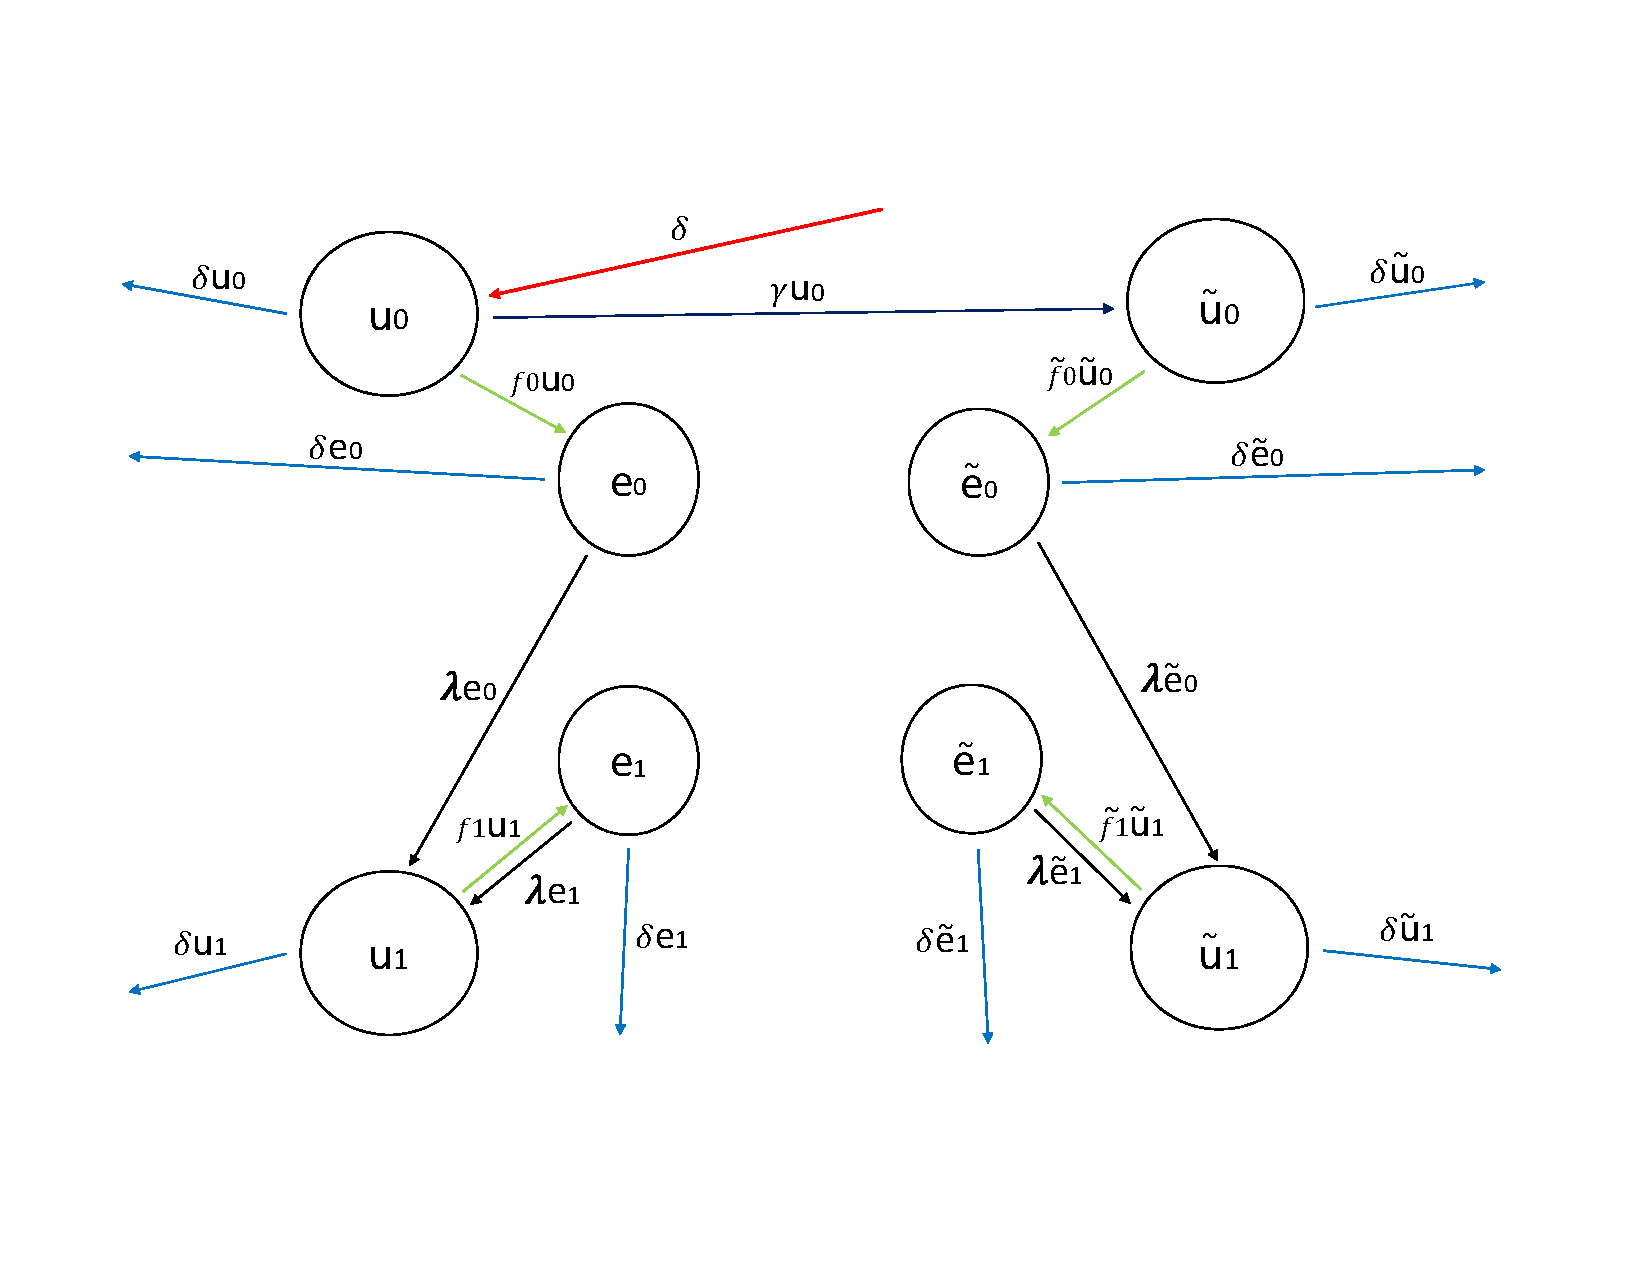
\includegraphics[scale=0.42]{empl_states.pdf}
        \end{figure}
\end{frame}


%----------------------------------------------------------------------------------------

%===============================================
\section{Key blocks} 
%===============================================
\begin{frame}{Beveridge curves}
\smallskip
\textbf{Equating inflows and outflows:}
\smallskip
\begin{align*}
    u_0 &= \frac{\delta}{\delta+\gamma+f_0} \\
    \tilde{u}_0 &= \frac{\gamma}{\delta+\tilde{f}_0} \cdot \frac{\delta}{\delta+\gamma+f_0} \\
    e_0 &= \frac{f_0}{\delta+\lambda} \cdot \frac{\delta}{\delta+\gamma+f_0} \\
    \tilde{e}_0 &= \frac{\tilde{f}_0}{\delta+\lambda} \cdot \frac{\gamma}{\delta + \tilde{f}_0} \cdot \frac{\delta}{\delta+\gamma+f_0} \\
    u_1 &= \frac{\lambda f_0}{(\gamma+\delta+f_0)(\delta+\lambda+f_1)} \\
     e_1 &= \frac{f_1}{\delta+\lambda} \cdot \frac{\lambda f_0}{(\gamma+\delta+f_0)(\delta+\lambda+f_1)} \\
     \tilde{u}_1 &= \frac{\lambda \gamma \tilde{f}_0}{(\delta+\tilde{f}_0)(\gamma+\delta+f_0)(\delta+\lambda+\tilde{f}_1)} \\
     \tilde{e}_1 &= \frac{\tilde{f}_1\lambda \gamma \tilde{f}_0}{(\delta+\lambda)(\delta+\tilde{f}_0)(\gamma+\delta+f_0)(\delta+\lambda+\tilde{f}_1)} 
\end{align*}

\end{frame}

\begin{frame}{Firms' value functions}
\begin{itemize}
\setlength\itemsep{1.8em}

    \item Free Entry/ Job Creation: 
    \smallskip
    \begin{equation*}
        c = q_0J_0 + \tilde{q}_0\tilde{J}_0 + q_1J_1 + \tilde{q}_1\tilde{J}_1
        \end{equation*}

 \item Values of employing different workers
 \smallskip
    \begin{align*}
    rJ_0 &= p-\kappa - w_0 - (\lambda + \delta) J_0 \\
    \smallskip
    r\tilde{J}_0 &= p-\kappa-\Tilde{\kappa}-\tilde{w}_0-(\lambda + \delta)\tilde{J}_0 \\
    \smallskip
    rJ_1 &= p-w_1-(\lambda + \delta)J_1 \\
    \smallskip
    r\tilde{J}_1 &=p-\tilde{\kappa}-\tilde{w}_1-(\lambda + \delta) \tilde{J}_1
\end{align*}

\end{itemize}
\end{frame}

%----------------------------------------------------------------------------------------

\begin{frame}{Workers' value functions}

\begin{itemize}
\setlength\itemsep{1.8em}
\item Employed
\smallskip
\begin{align*}
    rW_0 &=w_0+\lambda(U_1-W_0)- \delta W_0 \\
    \smallskip
    rW_1 &=w_1+\lambda(U_1-W_1)- \delta W_1 \\
    \smallskip
    r\tilde{W}_0 &=\tilde{w}_0+\lambda(\tilde{U}_1-\tilde{W}_0)- \delta \tilde{W}_0 \\
    \smallskip
    r\tilde{W}_1 &=\tilde{w}_1+\lambda(\tilde{U}_1-\tilde{W}_1)- \delta \tilde{W}_1
\end{align*}

\item Unemployed
\smallskip
\begin{align*}
    rU_0 &=z+f_0(W_0-U_0)+\gamma(\tilde{U}_0-U_0) - \delta U_0 \\
    \smallskip
    r\tilde{U}_0 &=z+\tilde{f}_0(\tilde{W}_0-\tilde{U}_0)- \delta \tilde{U}_0 \\
    \smallskip
     r U_{1} &=z+f_1(W_1-U_1)- \delta U_1 \\
     \smallskip
    r\tilde{U}_1 &=z+\tilde{f}_1(\tilde{W}_1-\tilde{U}_1)- \delta \tilde{U}_1
\end{align*}
\end{itemize}
\end{frame}


%----------------------------------------------------------------------------------------

\begin{frame}{Bargaining I}
\begin{itemize}

    \item Bargaining in type 1 meeting
    \begin{equation*}
    (1-\eta)(W_1-U_1) = \eta J_1 \implies w_1 = \frac{\eta p (r+\lambda+\delta+f_1)+(1-\eta)z(r+\lambda+\delta)}{r+\lambda+\delta + \eta f_1}
    \end{equation*}
    
     \item Bargaining in type $\tilde{1}$ meeting
    \begin{equation*}
        (1-\eta)(\tilde{W}_1-\tilde{U}_1) = \eta \tilde{J}_1 \implies \tilde{w}_1 = \frac{\eta (p-\Tilde{\kappa}) (r+\lambda+\delta+\tilde{f}_1)+(1-\eta)z(r+\lambda+\delta)}{r+\lambda+\delta + \eta \tilde{f}_1}
    \end{equation*}
    
    \item Bargaining in type $\tilde{0}$ meeting
    \begin{equation*}
    \begin{split}
        (1-\eta)(\tilde{W}_0-\tilde{U}_0) = \eta \tilde{J}_0 \implies \tilde{w}_0 = \frac{1}{r+\delta+\eta \tilde{f}_0} \Big[ \eta(p-\kappa-\tilde{\kappa})(r+\delta+\tilde{f}_0) + \\ + (1-\eta)z \frac{(r+\delta+\lambda) (r+\delta+\tilde{f}_1)} {r+\delta+\lambda+\tilde{f}_1}-\frac{\lambda(1-\eta)\tilde{f}_1}{r+\delta+\lambda+\tilde{f}_1} \tilde{w}_{1} \Big]
        \end{split}
    \end{equation*}
    
\end{itemize}
\end{frame}



%----------------------------------------------------------------------------------------

\begin{frame}{Bargaining II}
\begin{itemize}
    \setlength\itemsep{1.8em}

     \item Bargaining in type 0 meeting
    \begin{equation*}
    \begin{split}
       (1-\eta)(W_0-U_0) = \eta J_0 \implies w_0 = \frac{r+\delta+\gamma +f_0}{r+\delta+\gamma+\eta f_0}\eta (p-\kappa) + \\ + \frac{(r+\lambda+\delta)(r+f_1+\delta)(r+\gamma+\delta)}{(r+\delta)(r+\delta+\gamma + \eta f_0)(r+\lambda+\delta+f_1)} (1-\eta) z + \\ + \frac{\gamma \tilde{f}_0}{(r+\delta)(r+\delta+\gamma + \eta f_0)}\eta(p-\kappa-\tilde{\kappa}-\tilde{w}_0) - \\ - \frac{(1-\eta)\lambda f_1 (r+\gamma+\delta)w_1}{(r+\delta)(r+\delta+\gamma + \eta f_0)(r+\lambda+\delta+f_1)} 
       \end{split}
    \end{equation*}


    \item Notice that $w_{1}$ enters negatively: new workers are willing to accept a lower wage to get access to their first job and a higher continuation value
    
\end{itemize}
\end{frame}




%===============================================
\section{Calibration} 
%===============================================

\begin{frame}{Early-career skill loss}
\begin{itemize}
\setlength\itemsep{1.8em} 
   
    \item Initial labor market conditions have persistent effects on young adults' earnings for 10-15 years (von Wachter, 2020) 

    \item Two recent studies focus on new workers:
    \smallskip
    \begin{itemize}
        \item Arellano-Bover (2022): workers who faced higher unemployment rates at ages 18 to 25 have lower skills at ages 36 to 59
        \smallskip
        \item Dinerstein, Megalokonomou and Yannelis (2022): show negative effects of the length of unemployment on teachers’ performance measured by students’ test scores
    \end{itemize}

    \item To translate this into wages we use Ortego Marti's (2016, 2017) estimates assuming $\gamma = 1/6$
\end{itemize}
\end{frame}

\begin{frame}{More data}
\begin{itemize}
\setlength\itemsep{1.8em} 
   
    \item Monthly CPS data 1994-2020
    \smallskip
    \begin{itemize}
        \item Average unemployment rate: 5.8\%
        \item Fraction of entrants in the unemployment pool: 9\%
        \item Fraction of LTU in the entrant pool: 28\%
    \end{itemize}

    \item Various surveys for training costs
    \smallskip
    \begin{itemize}
        \item Training Industry Report: \$1,075 in 2017, \$1,071 in 2021
        \item Association for talent development: \$1,252 in 2016
        \item Masui (2022) calibrates them at a value comparable to vacancy costs 
    \end{itemize}

    \item We set a target of \$1,000 2017 dollars which results in 0.8\% of GDP
    \smallskip
    \begin{itemize}
        \item Vacancy costs are estimated 1-2\% of GDP in the literature
    \end{itemize} 

    \item Finally, we use Hall and Milgrom's (2008) 71\% for $z/\mathbb{E}(p)$ (midpoint of Chodorow-Reich and Karabarbounis, 2016)
\end{itemize}
\end{frame}

\begin{frame}{Parameter values}
\begin{table}
\centering
%\begin{adjustbox}{width=0.75\columnwidth,center}
 \begin{tabular}{|c | c | c|} 
 \hline
 \textbf{Parameter} & \textbf{Description} & \textbf{Value}\\  
 \hline
  $p$  & Productivity    & 1   \\ 
  $r$   & Interest Rate   & 0.0042  \\
  $\alpha$ & Matching Elasticity & 0.72  \\
  $\eta$ & Worker Bargaining Power  & 0.72  \\
  $\gamma$ & Skill Loss Rate & 1/6  \\   
 \hline
  $\delta$  & Worker Exit Rate    & 0.0023   \\ 
  $\lambda$  & Separation Rate    & 0.0341  \\
  $c$ & Vacancy Cost & 1.71  \\
  $z$ & Unemployment Value  & 0.65  \\
  $\kappa$  & Training Cost & 0.11  \\ 
  $ \tilde{\kappa}$  & Skill Loss Scar & 0.07  \\ [1ex]  
 \hline
 \end{tabular}
%\end{adjustbox}
\end{table} 
\end{frame}


%===============================================
\section{Results} 
%===============================================

\begin{frame}{Policy interventions}
\begin{enumerate}
\setlength\itemsep{1.6em}
    \item Ranking is not allowed by government regulation
    \smallskip
    \begin{itemize}
        \item Standard DMP with heterogeneous workers in a common labor market 
    \end{itemize}
    \item Government subsidizes firms to cover for training costs and skill loss
    \smallskip
    \begin{itemize}
        \item Government takes away $\tau$ from all matches
        \item Firms are indifferent between workers
    \end{itemize}
        \item Internships: new workers are paid an exogenous wage
        \smallskip
    \begin{itemize}
        \item Ranking is not allowed 
        \item Fix $\tilde{w_{0}} = z$ and compute the effects of different $w_{0}$
    \end{itemize}
    \item Government subsidizes firms enough to prefer entrants
    \smallskip
    \begin{itemize}
        \item Subsidy $\sigma_0=\kappa(1+\rho)$ to every firm that hires a type-0 worker 
        \item Flat tax $\tau = \kappa(1+\rho)e_0/e$
    \end{itemize}
\end{enumerate}
\vspace{0.25cm}
Welfare $=$ aggregate surplus - vacancy costs 

\vspace{0.1cm}
Short- vs Long-run Productivity trade off: less hires of new workers $\Rightarrow$ more matches without training costs but greater skill loss for entrants
\end{frame}

\begin{frame}{Baseline economy with ranking}
\begin{itemize}
\setlength\itemsep{1.5em}

\item Welfare level is 0.9398

\item Unemployment rate is 5.8\%
    
    \item Job finding rates
    \smallskip
    \begin{itemize}
    %\setlength\itemsep{1.25em}
        \item $\tilde{f_{0}} = 0.42$ 
        \item $f_{0} = 0.43$
        \item $\tilde{f_{1}} = 0.46$ 
        \item $f_{1} = 0.69$
    \end{itemize}

    \item Wages
    \smallskip
    \begin{itemize}
    %\setlength\itemsep{1.25em}
        \item $\tilde{w_{0}} = 0.82$ 
        \item $w_{0} = 0.66$ (non-scarred workers accept lower wages to get out of the bad state)
        \item $\tilde{w_{1}} = 0.92$ 
        \item $w_{1} = 0.99$
    \end{itemize}
        
\end{itemize}
 
\end{frame}


\begin{frame}{Intervention 1: Ranking ban}
\begin{itemize}
\setlength\itemsep{1.5em}

\item Welfare level is 0.9433 (from 0.9398); firms rank too much!

\item Unemployment rate is 6.9\% (from 5.8\%)
    
\item Job finding rate is the same for all workers: $f = 0.49$
\smallskip
    \begin{itemize}
        \item Increases for all workers other than the experienced ones without scar
    \end{itemize}

\item Wages
    \smallskip
    \begin{itemize}
        \item $\tilde{w_{0}} = 0.81$ 
        \item $w_{0} = 0.84$ (big winners)
        \item $\tilde{w_{1}} = 0.92$ 
        \item $w_{0} = 0.99$
    \end{itemize}

    \item Economics: we ``force'' firms to incur larger training costs
    \smallskip
    \begin{itemize}
        \item less entry $\Rightarrow$ aggregate unemployment increases 
        \item more matches with inexperienced workers $\Rightarrow$ short-run productivity decreases 
        \item in general equilibrium, however, welfare is higher!
        \item entrants' unemployment duration is shorter $\Rightarrow$ less likely to suffer skill loss
    \end{itemize}
        
\end{itemize}
 
\end{frame}


\begin{frame}{Intervention 2: Government subsidies}
\begin{itemize}
\setlength\itemsep{1.8em}

\item Welfare level is 0.9427; not as effective as ranking ban

\item Unemployment rate is 7.2\% (an even greater increase)
    
\item Job finding rate is the same for all workers: $f = 0.47$
    \begin{itemize}
        \item Increases for all workers other than the experienced ones without scar
    \end{itemize}

\item Wage is the same for all workers: $w = 0.96$
    \begin{itemize}
        \item Increases for all workers other than the experienced ones without scar
    \end{itemize}

    \item Same economics as the government ban
    \begin{itemize}
        \item The model that bans ranking delivers higher welfare
        \item It avoids the use of additional distortionary taxes
    \end{itemize}
        
\end{itemize}
 
\end{frame}


\begin{frame}{Intervention 3: Internships}
\begin{columns}
\column{0.5\textwidth}
\begin{minipage}[c][0.5\textheight][c]{\linewidth}
  \centering
  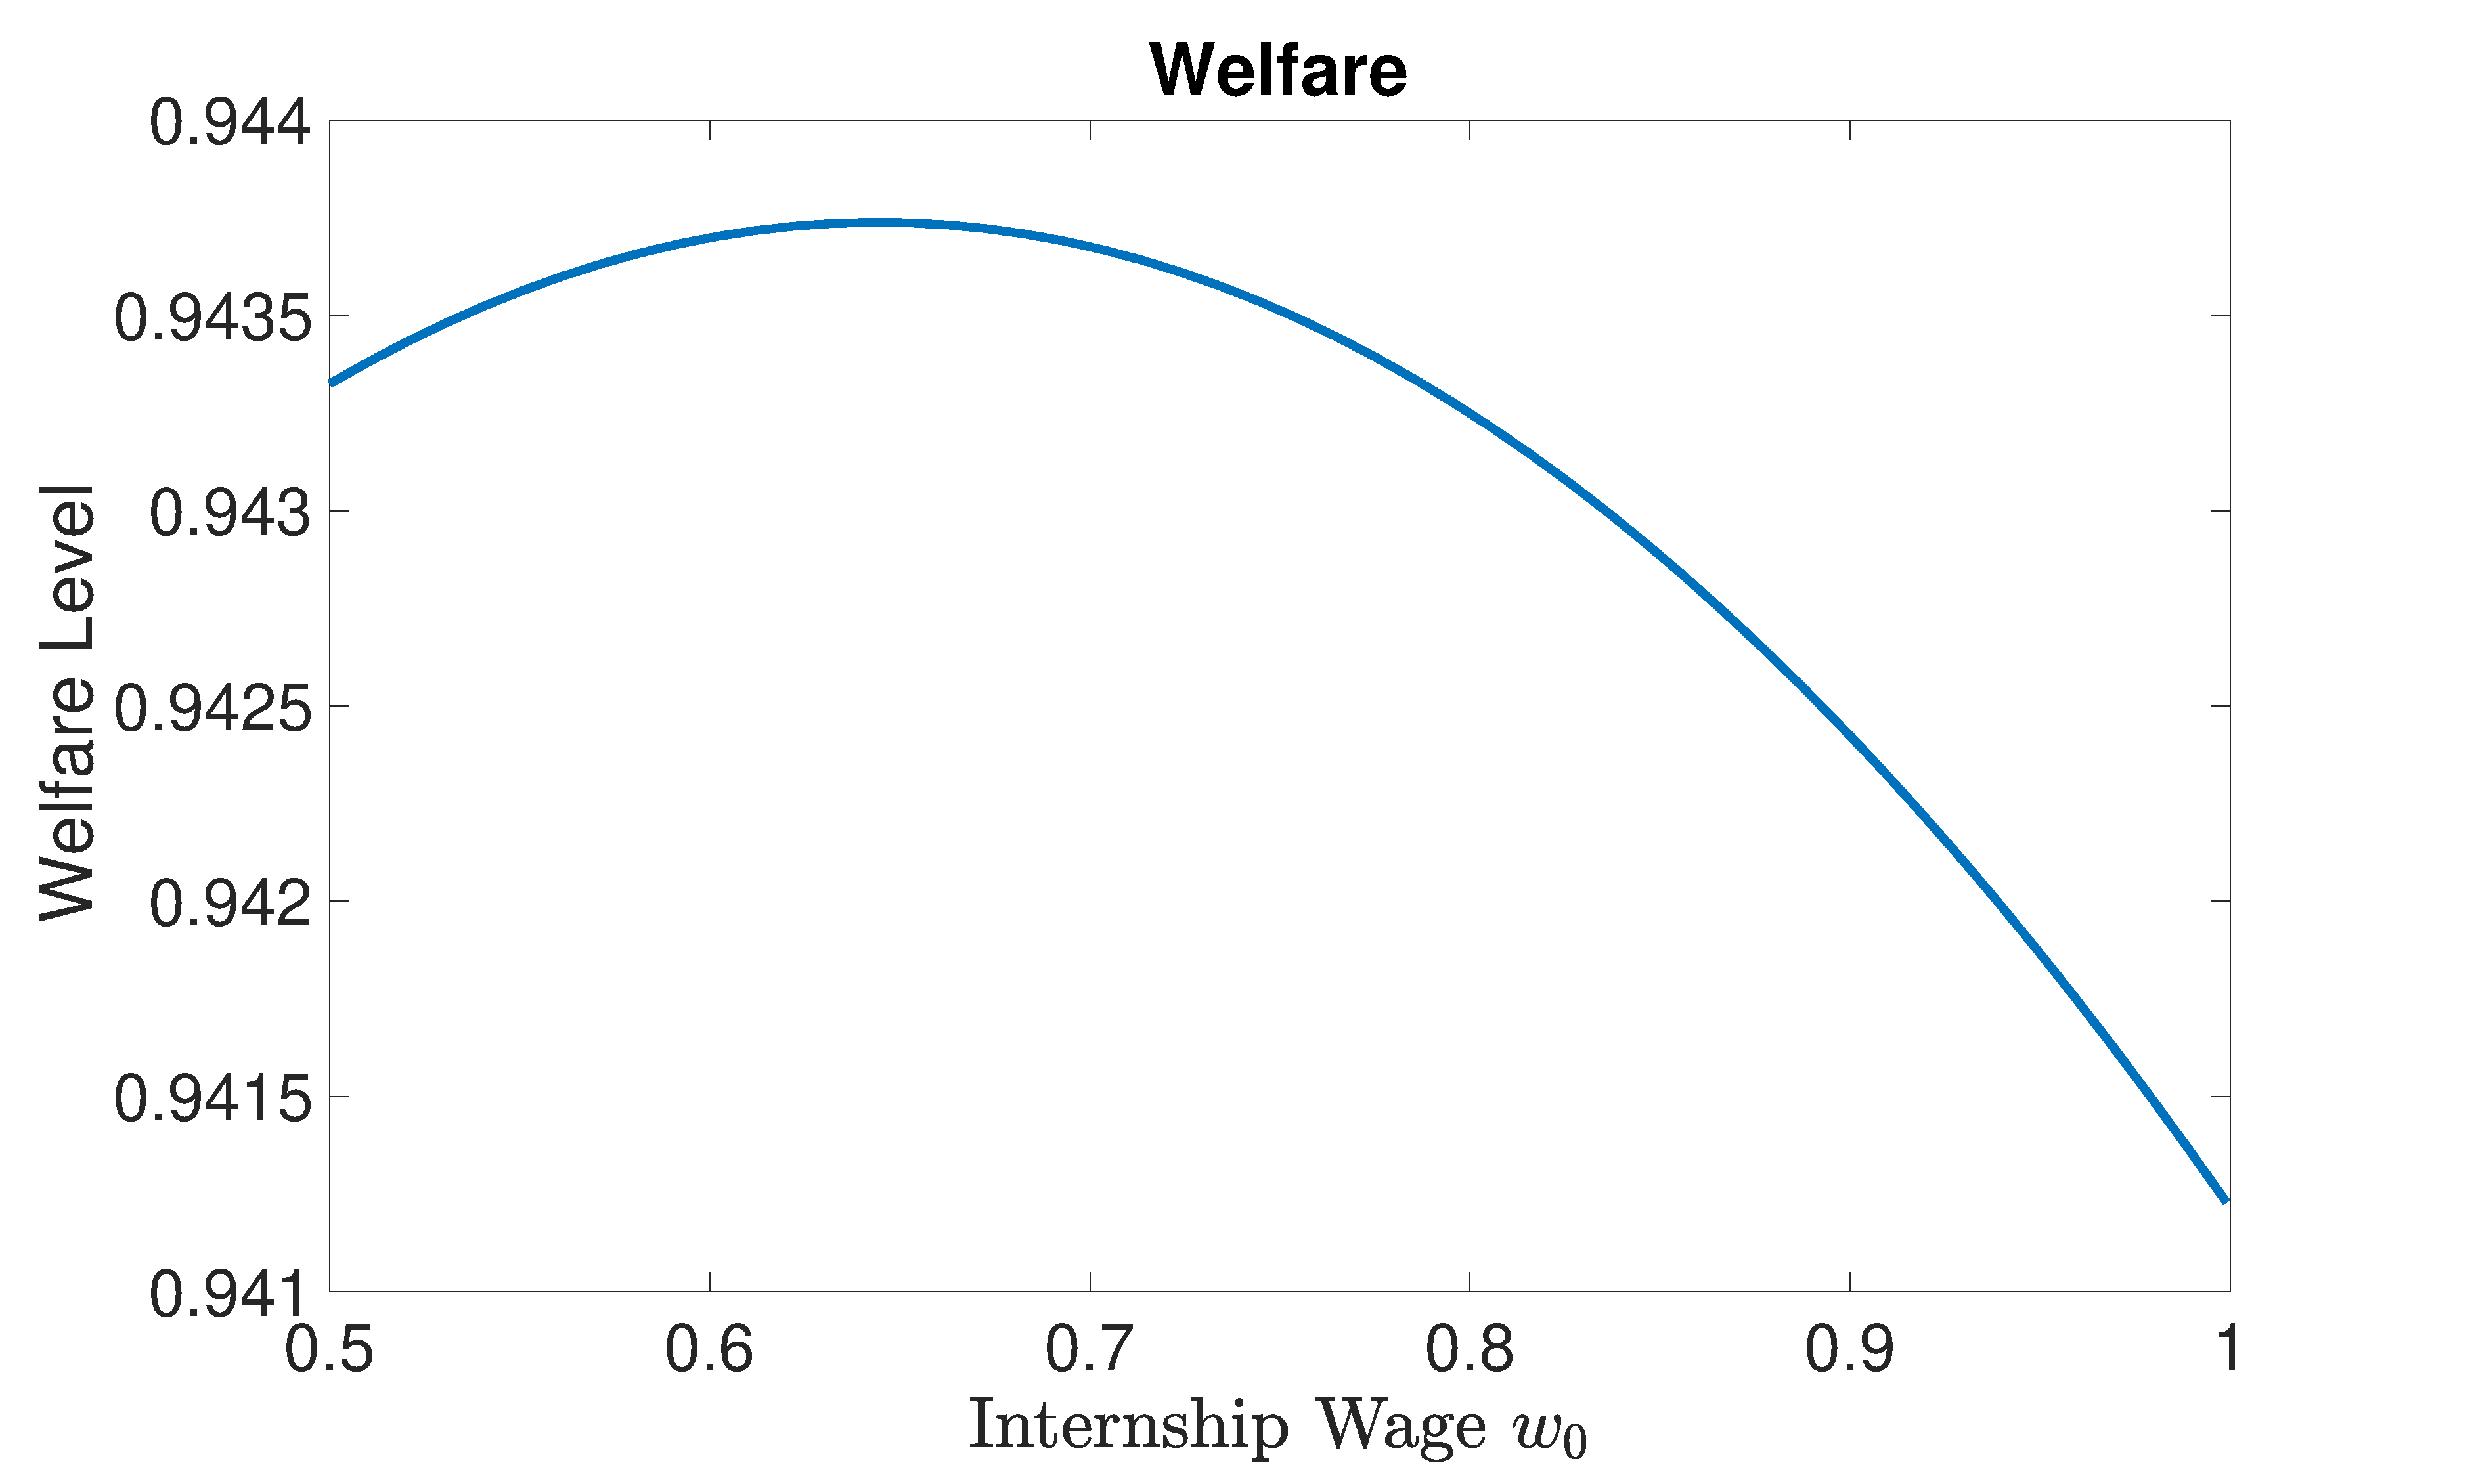
\includegraphics[scale=0.07]{welfare_intern.eps}
\end{minipage}
\begin{minipage}[c][0.5\textheight][c]{\linewidth}
  \centering
  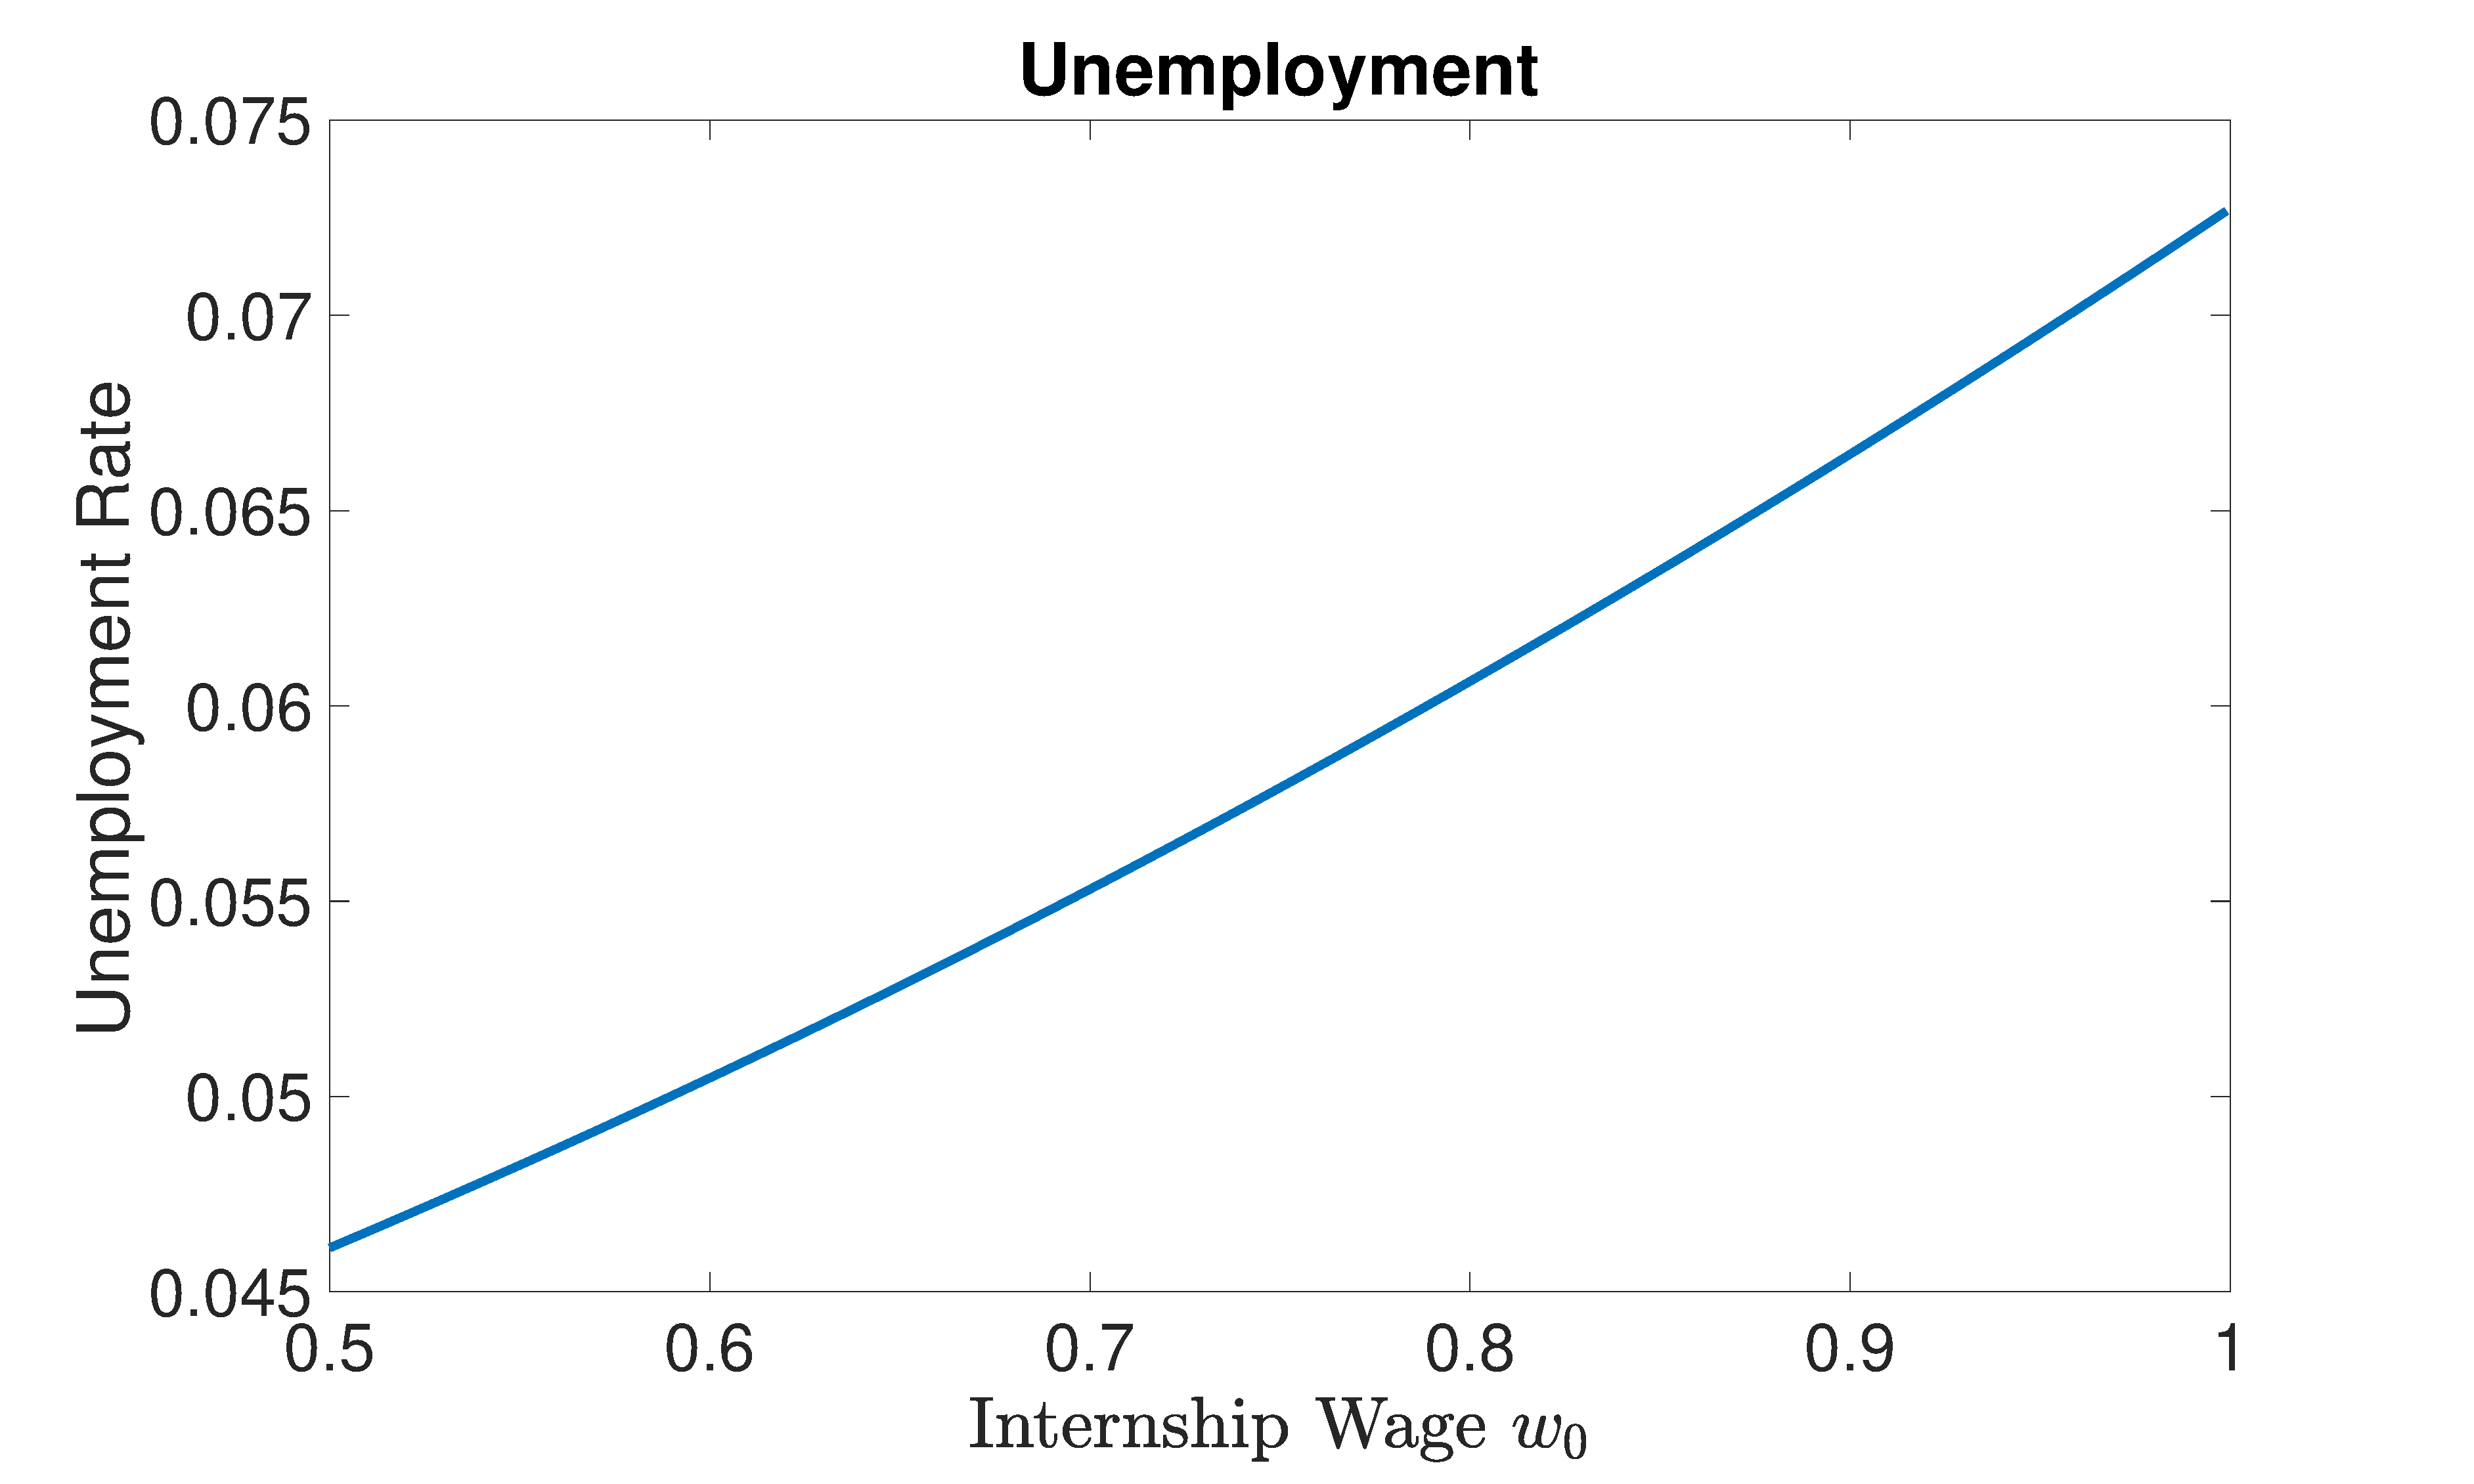
\includegraphics[scale=0.07]{urate_intern.eps}
\end{minipage}
\column{0.5\textwidth}
\begin{minipage}[c][0.5\textheight][c]{\linewidth}
  \begin{itemize}
  \item $\tilde{w_{0}} = z$
  \item Welfare always greater than ranking, max at 0.9437 with $w_{0} = 0.82$
  \item Too low $w_{0}$ $\Rightarrow$ entrants too cheap, large training and vacancy costs
  \item Too high $w_{0}$ $\Rightarrow$ back to main channel, large skill losses
  \end{itemize}
\end{minipage}
\begin{minipage}[c][0.5\textheight][c]{\linewidth}
  \centering
  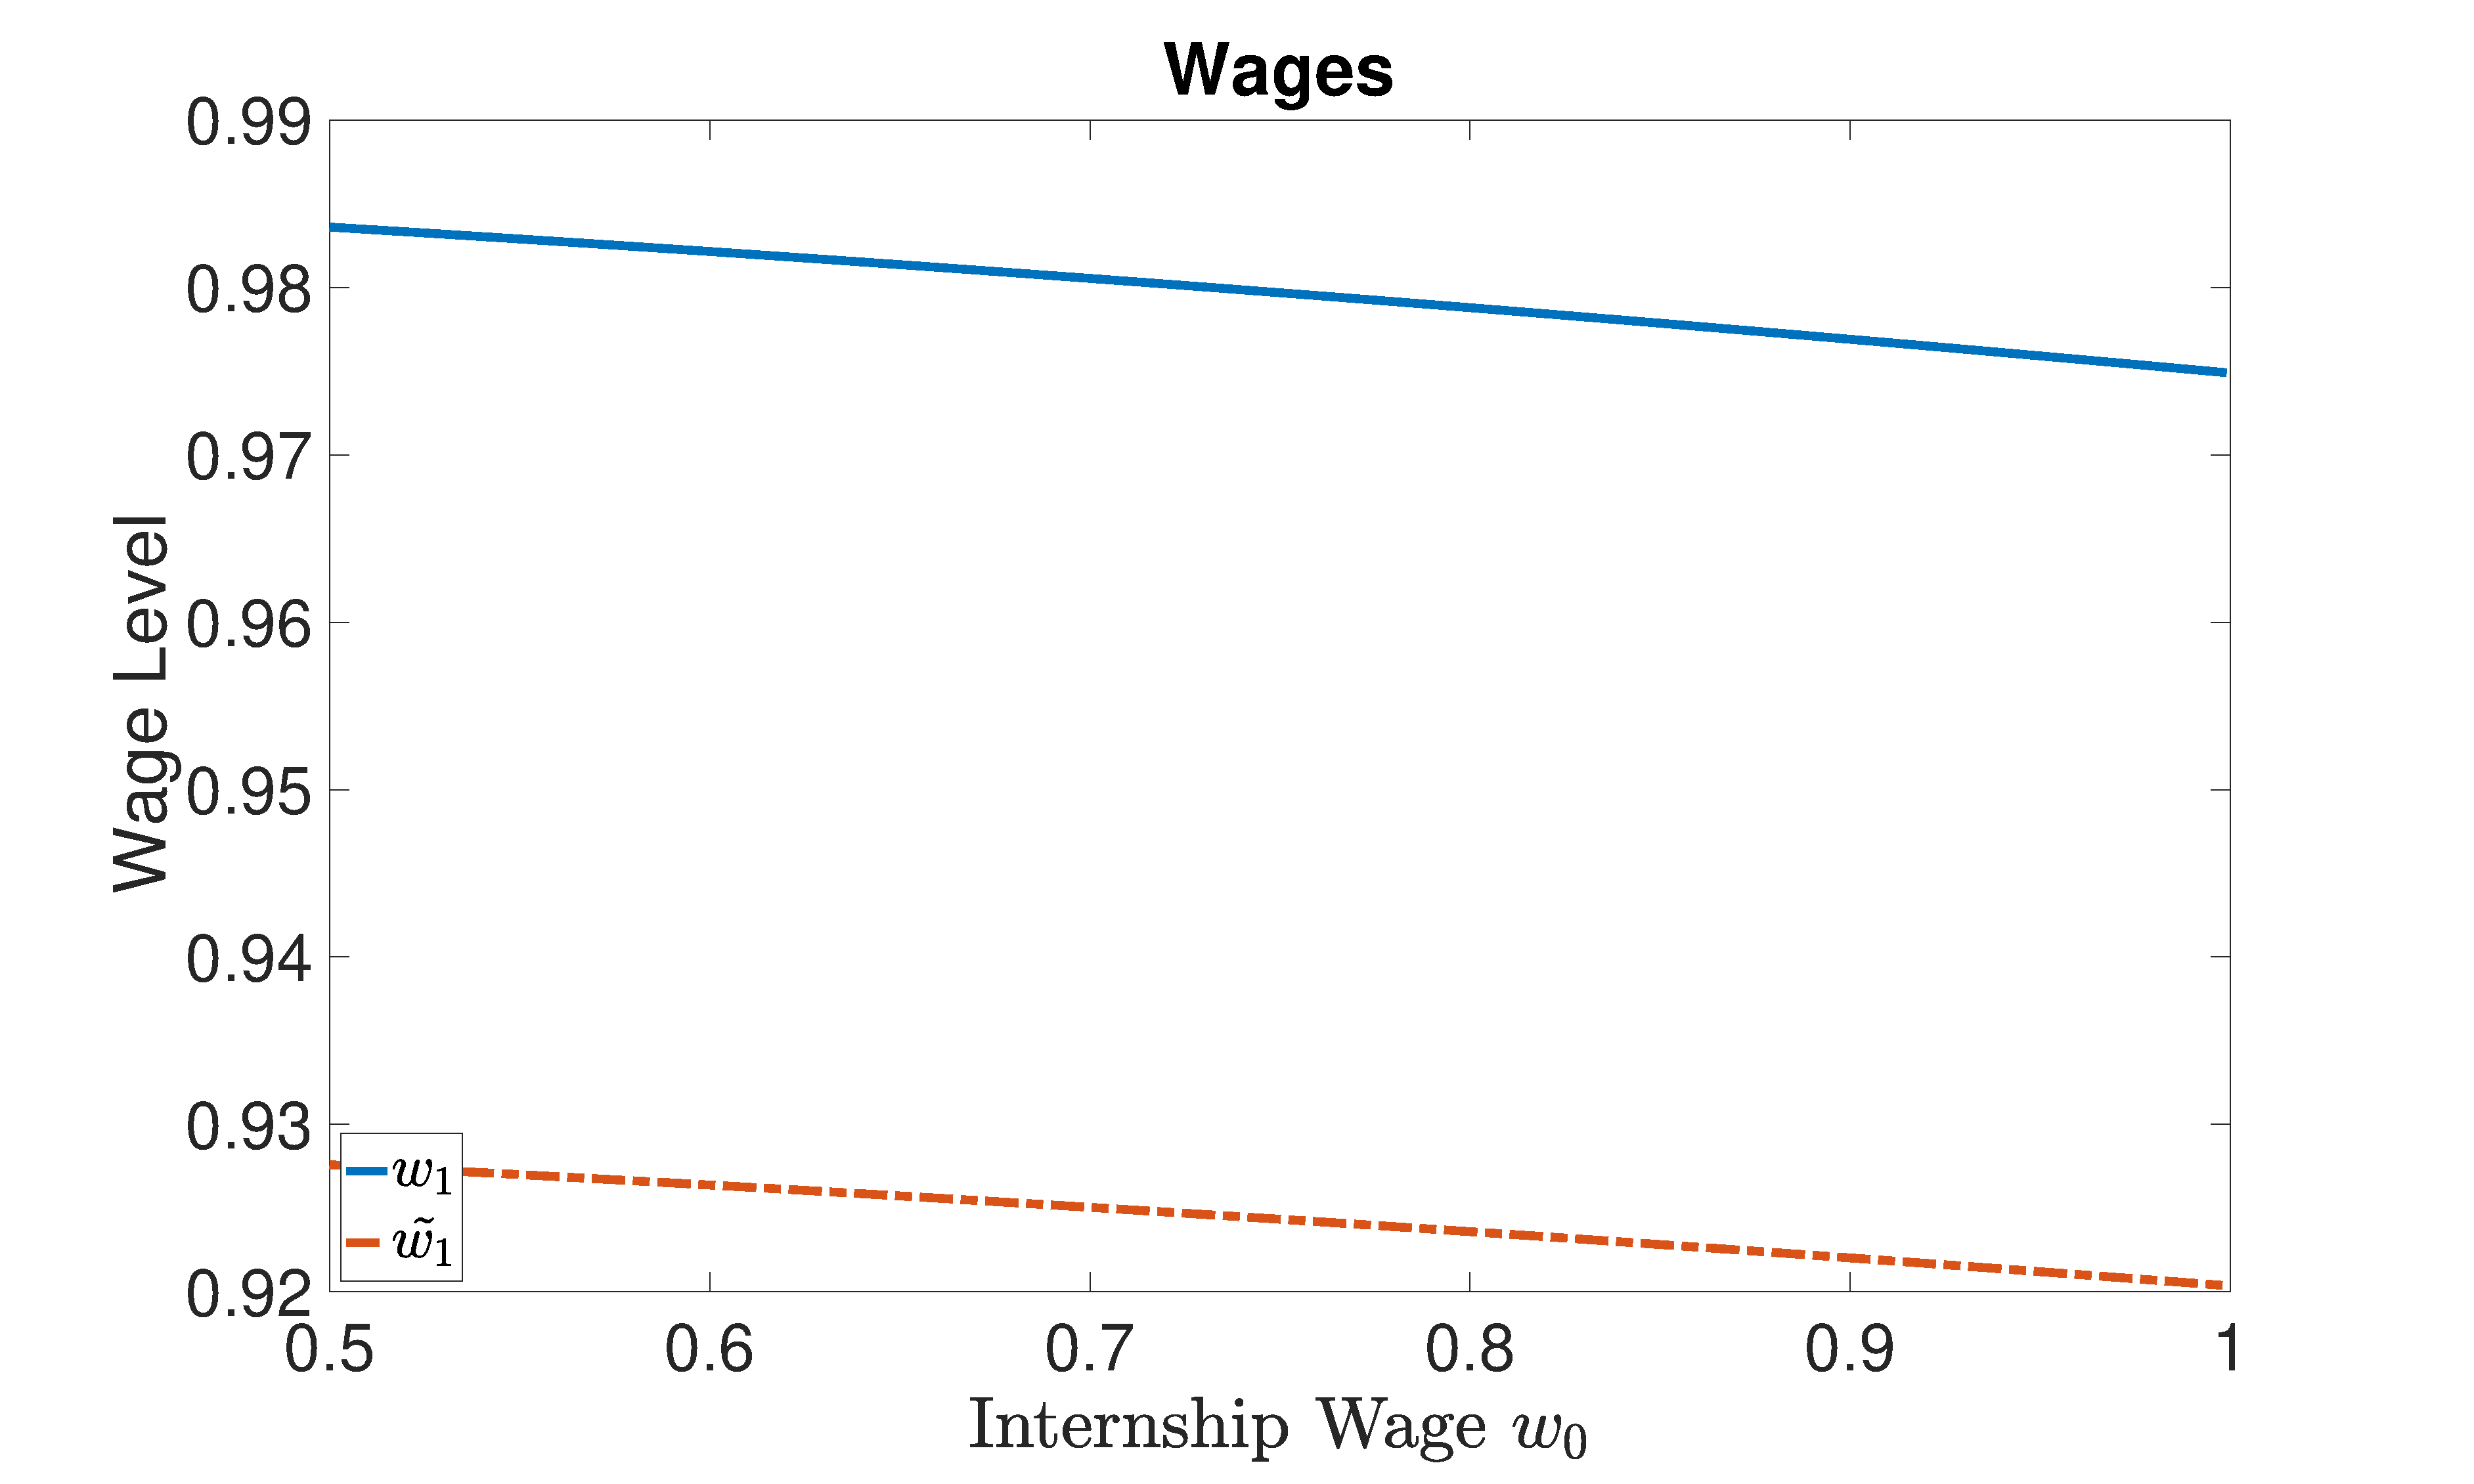
\includegraphics[scale=0.07]{wages_intern.eps}
\end{minipage}
\end{columns}
 
\end{frame}



\begin{frame}{Intervention 4: Type-0 Bias}
\begin{itemize}
\setlength\itemsep{1.8em}

\item Welfare level is 0.9531: 1.42\% increase, three times more effective than internships!

\item Unemployment rate is 6.52\% (in between internships and other interventions)
    
\item Raises $f_{0}$ almost four times: directly confronts the issue of entrants' long unemployment duration

\item Youth Employment Initiative: €8.9 billion program (2014-2020) to directly finance young workers' apprenticeships, traineeships, job placements, and further education within 4 months of leaving school or becoming unemployed

\item Based on our results, interventions of this kind are expected to have positive welfare gains even if they raise aggregate unemployment
        
\end{itemize}
 
\end{frame}

%===============================================
\section{Conclusion} 
%===============================================

\begin{frame}
\frametitle{Conclusion}
   \begin{itemize}
\setlength\itemsep{1.8em}
    \item Built a DMP model with entrants and experienced workers to study the implications of firms' preference for experienced workers

    \item In the model, firms who hire entrants provide a public service but are not compensated for it
    \smallskip
    \begin{itemize}
    \item Hence, they rank experienced over new workers
    \end{itemize}
    
    \item \textbf{Trade off}: more experienced hires have lower training costs and larger match surplus but increase entrants' unemployment duration leading to larger skill losses
    
    \item We evaluated four interventions with the calibrated model
    \smallskip
    \begin{itemize}
    \item Ranking ban, government subsidies, internships, type-0 bias
    \item Ranking equilibrium has lower welfare than all government interventions
    \item Internships are welfare-enhancing; optimal entrant wages at intermediate levels
    \item Type-0 bias delivers the largest welfare gains
    \end{itemize}

\end{itemize}
\end{frame}




\begin{frame}
\centering
\huge{Thank you!}
\end{frame}


%===============================================
\section{Appendix} 
%===============================================

\begin{frame}
\frametitle{Job Finding Rates Workers 16-64}
\begin{figure}
\centering
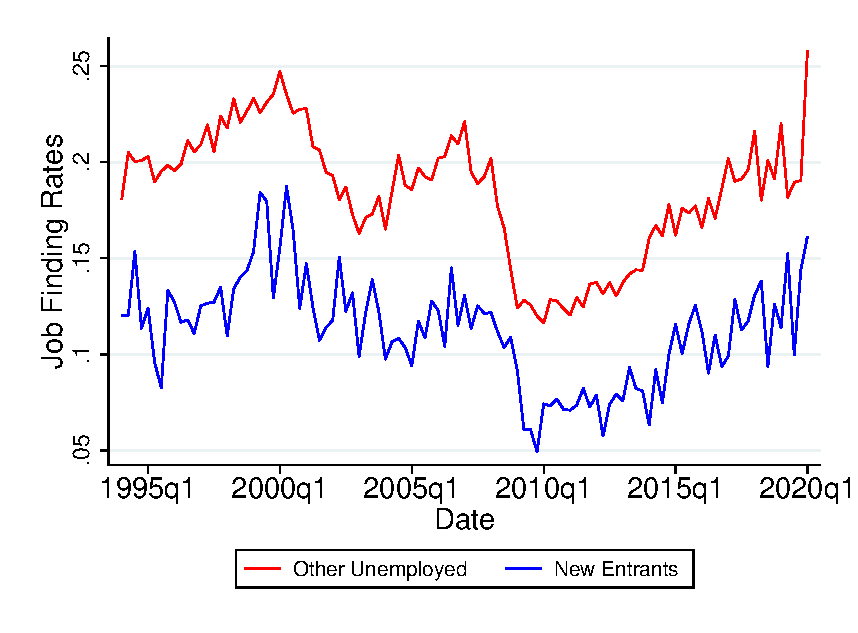
\includegraphics[width=0.85\textwidth]{JFR_all.eps}
\end{figure}
\hypertarget{jfr}{}
\end{frame}

\begin{frame}
\frametitle{Job Finding Rates Workers 16-24}
\begin{figure}
\centering
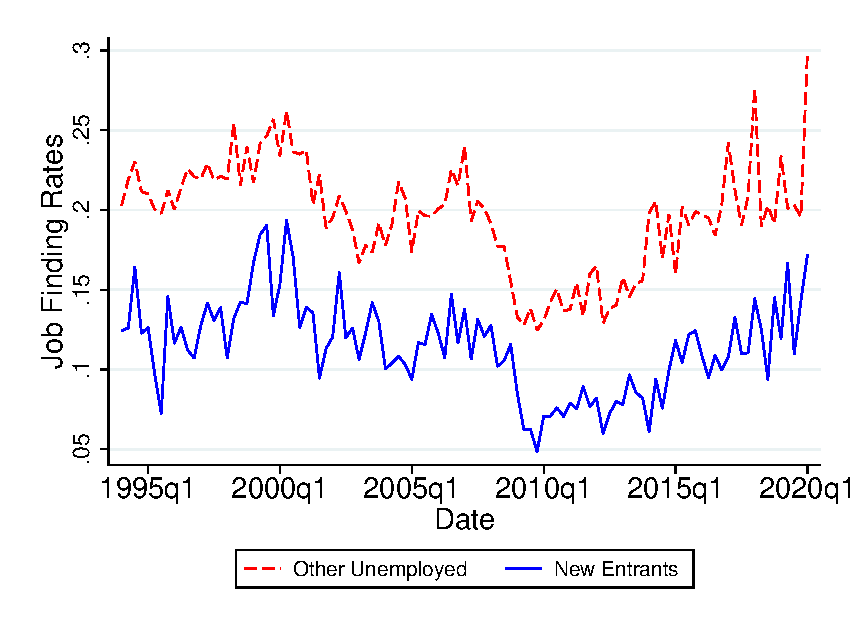
\includegraphics[width=0.85\textwidth]{JFR_16_24.eps}
\end{figure}
\hyperlink{flow_jfr}{\beamerbutton{Back to Intro}} 
\end{frame}





\end{document}